\documentclass[11pt]{article}

%-----------------------------------------------------------------------
% PACKAGES
%-----------------------------------------------------------------------
\usepackage[utf8]{inputenc}      % Encodes input in UTF-8
\usepackage[T1]{fontenc}         % Better handling of diacritics
\usepackage{lmodern}             % Latin modern font
\usepackage{amsmath,amssymb}     % Math symbols and environments
\usepackage{amsthm}              % Theorem-like environments
\usepackage{graphicx}            % For including figures
\usepackage{hyperref}            % Hyperlinks in PDF
\usepackage{caption}             % Better captions for figures/tables
\usepackage{cite}                % Better citation handling
\usepackage{geometry}            % Adjust page margins
\geometry{margin=1in}

%-----------------------------------------------------------------------
% TITLE, AUTHOR, AND DATE
%-----------------------------------------------------------------------
\title{\textbf{A Gentle Introduction to Coordinate Frame Conversions}}
\author{C. Padwick}
\date{\today}

%-----------------------------------------------------------------------
% CUSTOM COMMANDS & ENVIRONMENTS (OPTIONAL)
%-----------------------------------------------------------------------
\newtheorem{theorem}{Theorem}[section]
\newtheorem{lemma}{Lemma}[section]
\newtheorem{proposition}{Proposition}[section]
\newtheorem{definition}{Definition}[section]

% Example macro to quickly typeset a 2D rotation matrix
\newcommand{\RtwoD}[1]{%
\begin{pmatrix}
\cos #1 & -\sin #1 \\
\sin #1 & \cos #1
\end{pmatrix}%
}

% Example macro to quickly typeset a 3D rotation matrix around the z-axis
\newcommand{\RthreeD}[1]{%
\begin{pmatrix}
\cos #1 & -\sin #1 & 0 \\
\sin #1 & \cos #1 & 0 \\
0       & 0       & 1
\end{pmatrix}%
}

%-----------------------------------------------------------------------
\begin{document}

% MAKE TITLE AND TABLE OF CONTENTS
\maketitle
\tableofcontents
\clearpage

%-----------------------------------------------------------------------
% ABSTRACT
%-----------------------------------------------------------------------
\begin{abstract}
Imagine you have a robot with a camera mounted on it.  The camera measures something of interest,
like the distance to the nearest chair or the distance to the nearest wall, and you 
want the robot to navigate to that object.  Since it is usually impossible to locate the
camera exactly at the origin of the robot, it is necessary to convert the distance from the
camera to the object into a distance from the robot.  This is called a coordinate frame conversion.  
Generally speaking this coordinate frame conversion consists of rotation and translation from the
camera frame to the robot frame. This document is a short introduction to Euclidean coordinate frame conversions.
This document provides a gentle introduction to coordinate transformations (rotations and translations)
with the intent of giving the reader a solid understanding of the fundamentals without needing
an advanced mathematics or engineering course in linear algebra.
\end{abstract}

%-----------------------------------------------------------------------
% 1. INTRODUCTION
%-----------------------------------------------------------------------
\section{Introduction}
\label{sec:intro}

Image this: you are building a robot for a First Robotics competition and your vision mentor says "we need 
to correct the apriltag vector detected by the vision system to align with the robot's coordinate frame."
If you don't know what this means, then you are reading the right document!

You don't need a familiarity with robotics to read this document.  The same concepts will
apply to any device which takes measurements in a given coordinate frame and those measurements
need to be converted to a different coordinate frame.  Rotation matrices are essential in many 
areas of mathematics, engineering, and computer science.  In this doc I'm going to go over
some basics and give a gentle introduction so you can get the working knowledge you need and
move on to more advanced topics later.

%-----------------------------------------------------------------------
% 2. Coordinate Frames and Vectors
%-----------------------------------------------------------------------
\section{Coordinate Frames and Vectors}
\label{sec:coordinateframes}

A coordinate frame is a set of vectors, or axes, which are orthogonal to each other.  Orthogonal
means the angle between any two axes is 90 degrees.  A simple 2D coordinate frame is shown in figure \ref{fig:cf1}.

\begin{figure}[h!]
    \centering
    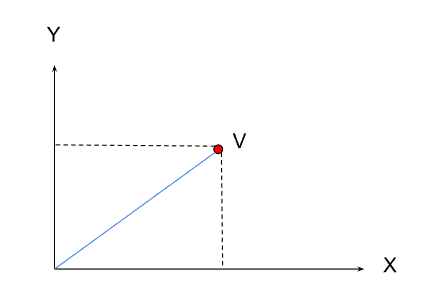
\includegraphics{figures/cf1.png}
    \caption{An 2D coordinate frame defined by X and Y.}
    \label{fig:cf1}
\end{figure}

The coordinate frame is useful because we can locate points in the coordinate frame by their X
and Y coordinates.  For example, the point V in figure \ref{fig:cf1} has an x and a y coordinate
that can be determined by its position on the coordinate frame.  In the figure these components
on the X and Y axes are shown by the dashed lines.

In terms of expressing the position of a point in the coordinate frame, we can write a vector as follows:

\begin{equation}
\vec{v} = 
\begin{bmatrix}
v_x \\
v_y
\end{bmatrix}.
\end{equation}

where \(v_x\) is the x-component of the vector and \(v_y\) is the y-component of the vector.  You can
compute the length of the vector easily too by taking the square root of the sum of the
squares of the components:

\begin{equation}    
|\vec{v}| = \sqrt{v_x^2 + v_y^2}.
\end{equation}

The extension to 3-dimensions or even N-dimensions is straight forward - you just add one more
component for each dimension.


%-----------------------------------------------------------------------
% 3. 2D ROTATION MATRICES
%-----------------------------------------------------------------------
\section{2D Rotation Matrices}
\label{sec:2d-rotation}

We’re going to work out some simple rotations in 2D so we can get some experience with
rotation matrices and how they work.  This can all be extended to 3D but it's easier to
visualize in 2D and nicer to start with.
\noindent
Let’s draw an X-Y axis in 2D and a rotated version of the axis, A-B, shown in figure \ref{fig:2d1}.
The rotation angle is $\theta$.  The rotation angle is positive, and is measured
counterclockwise.  For simplicity let’s set the length of A and B both to 1, 
.e.g \begin{equation} |A| = |B| = 1\end{equation}.

\begin{figure}[h!]
    \centering
    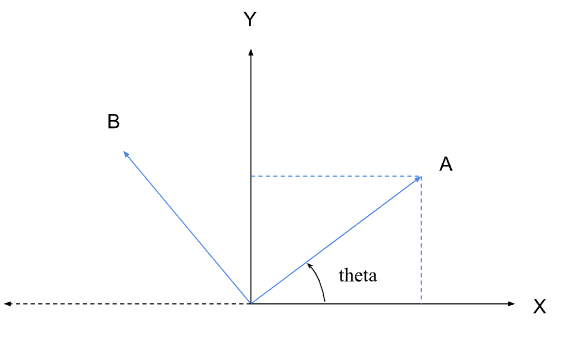
\includegraphics{figures/2d1.png}
    \caption{An 2D coordinate frame defined by X and Y, and a rotated version of the axis denoted by A-B.}
    \label{fig:2d1}
\end{figure}

Let's ask the following question: How do we get the coordinates of the points A and B
in the X-Y frame?  We are given the angle of rotation $\theta$.  We need to compute
the X-Y coordinates of each point A and B in the X-Y frame.

\noindent

Let's start with the point A.  From trigonometry we can figure out the X-Y coordinates
of A by noticing $cos(\theta) = x / |A|$ or $x = cos(\theta) * |A|$.  Since we said
that $|A| = 1$, we can just write $x = cos(\theta)$.  Similarly, we can figure out
the y coordinate of A by noticing that $sin(\theta) = y / |A|$ or $y = sin(\theta) * |A|$,
and we can just write $y = sin(\theta)$.  This gives us the X-Y
coordinates of A as:
\begin{equation}
    \vec{A} = 
    \begin{bmatrix}
    cos(\theta) \\
    sin(\theta)
    \end{bmatrix}.
\end{equation}

We can do the same for the point B.  We can see that the X coordinate of B is going to be
negative since it interects with the negative X axis.  We can do the same thing we did 
for the A coordinate, except this time we see that $sin(\theta) = -x / |B|$ or 
$x = -sin(\theta) * |B|$ => $x = -sin(\theta)$.  Take a moment and study the
diagram and convince yourself that this is true.  The y-coordinate of B is going to be
$cos(\theta) = y / |B|$ or $y = cos(\theta) * |B|$ => $y = cos(\theta)$.  Pause for a
few moments and study the diagram and convince yourself that this is true.

Writing out the coordinates B, we get:
\begin{equation}
    \vec{B} = 
    \begin{bmatrix}
    -sin(\theta) \\
    cos(\theta)
    \end{bmatrix}.
\end{equation}

If you wanted to express these points as vectors in the X-Y frame, you could write them 
as:

\begin{equation}
    \vec{A} = sin(\theta) \hat{x} + cos(\theta) \hat{y}
\end{equation}

\begin{equation}
    \vec{B} = -sin(\theta) \hat{x} + cos(\theta) \hat{y}
\end{equation}

The $\hat{x}$ and $\hat{y}$ are unit vectors in the X-Y frame.  They are aligned with the
X and Y axes respectively but have unit length.

\subsection{Representing The Rotation As A Matrix}

Now that we have the coordinates of A and B, we can represent the rotation as a matrix.  This
is actually quite simple.  We can write the rotation matrix as:
\begin{equation}
    R(\theta) = 
    \begin{bmatrix}
    cos(\theta) & -sin(\theta) \\
    sin(\theta) & cos(\theta)
    \end{bmatrix}.
\end{equation}

If you look at the entries of the matrix, you can recognize that we have taken the equation 
for $\vec{A}$ and put the X-Y coordinates into the first column.  The X coordinate goes in
the first row and the Y coordinate goes in the second row.  For the second column, we have
taken the equation for $\vec{B}$ and put the X-Y coordinates into the second column.
The X coordinate goes in the first row and the Y coordinate goes in the second row.

You might ask, why would we do this?  Why not just use the equations for $\vec{A}$ and $\vec{B}$ above?
It is customary to write something like "it turns out that we can use the rotation matrix more
easily and more efficiently".  It turns out that is true!

\subsection{Primer on Matrix/Vector Multiplication}

Ok, now let’s multiply a vector by a matrix.  In case you haven’t done this before, here is 
a quick primer on the rules of matrix multiplication:

\begin{itemize}
    \item When you multiply a vector by a matrix, the vector has to have the same number
of rows as the matrix has columns.  In this case we’ll express the vector as a column vector
with 2 rows and 1 column.  The matrix has 2 rows and 2 columns so we can multiply it by a 2x1 vector.

    \item When we multiply a vector by a matrix, as long as the vector has the same number of rows 
    as the matrix has columns, we get a vector of the same size as the input vector.  Since our vector 
    has 2 elements, the result will have two elements as well.

    \item When we’re multiplying a matrix and a vector, we start at the first row of the matrix 
    and multiply the column elements of the matrix by the rows of the vector and add them.  We put that
    result in the first element of the result vector.  We then move on to the second row of the matrix
    and multiply the column elements of the second row of the matrix by the rows of the vector and add them.  We put that
    result in the second element of the result vector.  We continue this process until we have computed 
    all the elements of the result vector.  In this case, the result vector will have 2 elements since
    we're only working with 2D rotation matrices.
\end{itemize}

Here is an example:
\begin{equation}
\begin{bmatrix} a_1 & a_2 \\
a_3 & a_4 \end{bmatrix} * \begin{bmatrix} v_1 \\v_2 \end{bmatrix} = \begin{bmatrix} a_1 v_1 + a_2 v_2 \\
a_3 v_1 + a_4 v_2 \end{bmatrix}
\end{equation}

\subsection{Applying The Rotation Matrix}

Alright, now that that is out of the way, let’s do a rotation.  Let’s say we have a vector in the A-B 
frame of reference, and this vector is just the A axis.  So the vector coordinates are just (1, 0) 
in the A-B frame of reference.  So let’s rotate this vector in the X-Y frame of reference:

\begin{equation}
    A_{xy-frame}=
    \begin{bmatrix} 
        cos(\theta) & -sin(\theta) \\
        sin(\theta) & cos(\theta) 
        \end{bmatrix}
    *
    \begin{bmatrix} 
        1 \\ 
        0 
    \end{bmatrix} = 
    \begin{bmatrix} 
        cos(\theta) + 0 \\
        sin(\theta) + 0 
    \end{bmatrix} 
    = 
    \begin{bmatrix} 
        cos(\theta) \\
        sin(\theta)
    \end{bmatrix}
    \end{equation}

This is the same answer we got before, so this is good news!
Let’s do it again, but for the B vector in the XY-frame:

\begin{equation}
    B_{xy-frame}=
    \begin{bmatrix} 
        cos(\theta) & -sin(\theta) \\
        sin(\theta) & cos(\theta) 
        \end{bmatrix}
    *
    \begin{bmatrix} 
        0 \\ 
        1 
    \end{bmatrix}
    = 
    \begin{bmatrix} 
        0 - sin(\theta) \\
        0 + cos(\theta)
    \end{bmatrix} 
    = 
    \begin{bmatrix} 
        -sin(\theta) \\
        cos(\theta)
    \end{bmatrix}
\end{equation}

This is the same result we got before, so this is good news!  It means our matrix multiply
approach actually works!

Ok, but why do we care?  What does this buy us?  This technique works for any vector in the A-B 
frame of reference.  So if someone gives us a vector in the A-B frame of reference, we can
multiply it by our 2D rotation matrix to get the vector in the X-Y frame of reference.
This is the first part of learning how to convert from one frame of reference to another!

%-----------------------------------------------------------------------
% 4. 3D ROTATION MATRICES
%-----------------------------------------------------------------------
\section{Extending to 3D Rotation Matrices}
\label{sec:3d-rotation}

Now that we have 2D rotation matrices, let’s extend them to 3D.  We said before that all we need
to do is add another component for the extra dimension.  Our 2D vectors now have 3 components,
and our 2D rotation matrices now have 3 rows and 3 columns, like this:

\begin{equation}
    \vec{v} = \begin{bmatrix} 
        v_x \\ 
        v_y \\
        v_z
    \end{bmatrix}
\end{equation}

\begin{equation}
    \begin{pmatrix}
        a_1 & a_2 & a_3 \\
        a_4 & a_5 & a_6 \\
        a_7 & a_8 & a_9
    \end{pmatrix}
\end{equation}

\subsection{Rotations About Each Axis}

It is possible to create a rotation matrix that rotates about the \(x\)-axis, the \(y\)-axis,
or the \(z\)-axis.  These matrices are simple to construct, and look very similar to their 2D
counterparts.

For instance, the rotation matrix around the \(z\)-axis is

\begin{equation}
    R_z(\theta) = 
    \begin{pmatrix}
        cos(\theta) & -sin(\theta) & 0 \\
        sin(\theta) & cos(\theta) & 0 \\
        0 & 0 & 1
    \end{pmatrix}
\end{equation}

You can recognize this as just the 2D rotation matrix about X-Y with some extra elements.
If you think about why this is, it actually makes sense.  In the 2D example we were
actually rotating about the z-axis, which faced out of the page.  When we rotate about
the z-axis the vectors only change in the X-Y plane.  So it makes sense that the matrix
would look this way in that the only components that change are the X-Y components.  Another
way to think about this is that the third column of the matrix is (0, 0, 1), which also
happens to the be coordinates of the z-axis.  Only the X-Y components change when whatever
rotate about the z-axis.

The rotation matrix around the \(y\)-axis is

\begin{equation}
    R_y(\gamma) = 
    \begin{pmatrix}
        cos(\gamma) & 0 & sin(\gamma) \\
        0 & 1 & 0 \\
        -sin(\gamma) & 0 & cos(\gamma) \\
        0 & 0 & 1
    \end{pmatrix}
\end{equation}

Here I have introduced another angle $\gamma$.  Notice that the second column of the matrix 
is (0, 1, 0), which also happens to the be coordinates of the y-axis.  When you rotate about
the y-axis the vectors only change in the X-Z plane.

The rotation matrix around the \(x\)-axis is

\begin{equation}
    R_x(\alpha) = 
    \begin{pmatrix}
        1 & 0 & 0 \\
        0 & cos(\alpha) & -sin(\alpha) \\
        0 & sin(\alpha) & cos(\alpha)
    \end{pmatrix}
\end{equation}

Here I have introduced another angle $\alpha$.  Notice that the first column of the matrix 
is (1, 0, 0), which also happens to the be coordinates of the x-axis.  When you rotate 
about the x-axis the vectors only change in the Y-Z plane.

\subsection{Worked Example}

Let's see if our rotations still work in 3D.  Let's take the same coordiate frame
as before in figure \ref{fig:2d1}.  Let's imagine that we have a vector Z in the X-Y frame,
and that vector points straight out of the page.  We'll call this frame X-Y-Z.  The frame
A-B also has a vector C that is aligned with the Z-axis and points straight out of the page.
We'll call this frame A-B-C.  So now we rotate A-B-C by angle $\theta$ around the Z-axis in the X-Y-Z frame,
and we want to compute the coordinates of the rotated A-B-C 

\subsection{Rotation About an Arbitrary Axis}
Discuss Rodrigues' rotation formula, quaternions, or Euler angles—whatever is relevant.

%-----------------------------------------------------------------------
% 5. PROPERTIES OF ROTATION MATRICES
%-----------------------------------------------------------------------
\section{Properties of Rotation Matrices}
\label{sec:properties}

Mention key properties like:
\begin{itemize}
    \item Orthogonality: \( R^\top R = I \)
    \item \(\det R = +1\)
    \item Composing rotations
    \item Relationship to \(\mathrm{SO}(n)\)
\end{itemize}

%-----------------------------------------------------------------------
% 6. APPLICATIONS
%-----------------------------------------------------------------------
\section{Applications}
\label{sec:applications}

Discuss practical uses:
\begin{itemize}
    \item Robotics
    \item Computer graphics
    \item Aerospace
    \item Image processing
\end{itemize}

%-----------------------------------------------------------------------
% 7. CONCLUSION
%-----------------------------------------------------------------------
\section{Conclusion}
\label{sec:conclusion}

Summarize key points. You may also mention limitations and open problems or suggest further reading.

%-----------------------------------------------------------------------
% REFERENCES
%-----------------------------------------------------------------------
\begin{thebibliography}{99}

\bibitem{ref:rotation-matrices}
Author Name, \emph{Title of Book or Paper}, Journal/Publisher, Year.

\bibitem{ref:so3}
Another Author, ``Interesting Insights Into 3D Rotations,'' Conference Proceedings, Year.

% Add more references as needed...

\end{thebibliography}

\end{document}
